\clearpage
\section{Soft- und Firmware}\label{sec:Soft-undFirmware}

Im folgenden Abschnitt wird das Konzept und die Umsetzung der Software für den Mesh Benchmark dokumentiert.
Dabei stand die Erfüllung der Anforderungen an die Software im Zentrum. Diese wurden in der Aufgabenstellung (siehe Anhang \ref{app:Aufgabenstellung}) sowie im Pflichtenheft (siehe Anhang \ref{app:Pflichtenheft}) vorgängig definiert. 

%\subsection{Anforderungen}\label{subsec:Software_Anforderungen}
%Wie im Abschnitt \ref{subsec:VergleichswerteundMessgrössenMesh} erwähnt, wurden die detaillierten Anforderungen an die Software bereits in der Aufgabenstellung (siehe Anhang \ref{app:Aufgabenstellung}) sowie im Pflichtenheft (siehe Anhang \ref{app:Pflichtenheft}) festgelegt.
%Im Fokus steht das erfassen der wichtigsten Messgrössen welche bereits in Abschnitt \ref{subsec:VergleichswerteundMessgrössenMesh} definiert wurden. 
%
%Die Erfassung der Messwerte muss in allen Mesh-Netzwerken möglich sein. Um die Messresultate vergleichen zu können müssen die gleichen Ausgangslagen vorliegen, sowie die selben Messmethoden angewendet werden. 


\subsection{Konzept}\label{subsec:Software_Konzept}

Um das Benchmark Konzept welches bereits im Abschnitt \ref{sec:BenchmarkKonzeptMeshNetzwerke} erläutert wurde, umsetzen zu können soll die Soft- und Firmware so aufgebaut sein, dass sie von allen Mesh-Stacks genutzt werden kann.
Zur Umsetzung der drei Mesh-Stacks auf der \textit{NRF-Plattform} wurden folgende \textit{Software Development Kits (SDK's)} eingesetzt. 

\begin{table}[h]
\centering
\begin{adjustbox}{width=1\textwidth}
\begin{tabular}{ll} 
\toprule
nRF Connect SDK & \begin{tabular}[t]{@{}l@{}}Die \textit{nRF Connect SDK} baut auf dem Zephyr-RTOS auf und unterstützt\\alle drei Mesh-Protokolle (Bluetooth-Mesh, Openthread und Zigbee).\\ Der Einsatz der SDK in einem End-Produkt wird jedoch noch nicht empfohlen. \cite{nordic_semi_welcome_to_the_nrf_connect_sdk_2020}\end{tabular} \\
\begin{tabular}[t]{@{}l@{}}nRF5 SDK for Thread\\and Zigbee\end{tabular} & \begin{tabular}[t]{@{}l@{}}Die \textit{nRF5 SDK for Thread and Zigbee} ist eine Software Bibliothek\\für die Entwicklung von Thread und Zigbee zertifizierten Produkten. \cite{nordic_semi_nrf_sdk_for_thread_and_zigbee_2020}\end{tabular} \\
nRF5 SDK for Mesh & \begin{tabular}[t]{@{}l@{}}Die \textit{nRF5 SDK for Mesh }ist eine Software Bibliothek\\für die Entwicklung von Bluetooth Mesh Lösungen. \cite{nordic_semi_nrf_sdk_for_mesh_2020}\end{tabular} \\
\bottomrule
\end{tabular}
\end{adjustbox}
\caption{Eingesetzte SDK's für die Umsetzung der Benchmark Firmware}
\label{tab:Eingesetzte SDKs}
\end{table}

Die Messungen sollten trotz der verschiedenen Bibliotheken möglichst einheitlich sein, um die Vergleichbarkeit nicht zu beeinträchtigen.
Daher wurde für das Benchmark Management eine eigene Kommunikationsebene entwickelt.
Diverse Module der P2P-Testinfrastruktur konnten dafür direkt oder indirekt verwendet werden.

\subsection{Umsetzung}\label{subsec:Software_Umsetzung}
Die Soft- und Firmware für die Mesh Benchmarks setzt sich aus mehreren Modulen zusammen. Die Tabelle \ref{tab:UebersichtSoftware} zeigt eine Übersicht der wichtigsten Module und deren Verwendung in den 3 Benchmark Teilen: BLE Mesh, Thread und Zigbee.
Gemeinsame Module auf Firmware Ebene sind im Ordner SharedLib im Github Repository\footnotemark\ zusammengefasst.

Jene Python Scripts für das Benchmark Management stehen im gleichnamigen Ordner ebenso auf dem Github Repository\footnotemark\ zur Verfügung.
Die Stack bezogenen Implementationen der Benchmark Firmware werden in den individuellen Teilen \ref{part:BluetoothMesh}, \ref{part:Thread} und \ref{part:Zigbee} behandelt.


\begin{table}[h]
\centering
\begin{tabular}{|l|l|l|c|} 
\hline
Library & Funktion & Modul & Referenz \\ 
\hline
\multirow{8}{*}{SharedLib} & Statemachine & bm\_statemachine.c & \ref{subsubsec:StatemachineSoftware} \\ 
\cline{2-4}
 & Timesync & bm\_timesync.c & \ref{subsubsec:Timesync}  \\ 
\cline{2-4}
 & Control & bm\_control.c & \ref{subsubsec:Control} \\ 
\cline{2-4}
 & Report & bm\_report.c & \ref{subsubsec:Report} \\ 
\cline{2-4}
 & Logging & bm\_log.c & \ref{subsubsec:Logging} \\ 
\cline{2-4}
 & Flash Save & bm\_flash\_save.c & \ref{subsubsec:FlashSave} \\ 
\cline{2-4}
 & CLI & bm\_cli.c & \ref{subsubsec:CLI} \\ 
\cline{2-4}
 & Low Layer Radio & bm\_radio.c & \ref{subsubsec:LowLevelRadio} \\ 
 \cline{2-4}
 & \begin{tabular}[c]{@{}l@{}}Random and Sequential \\ Traffic Generator  \end{tabular} & bm\_rand.c & \ref{subsubsec:TrafficGenerator} \\ 
\hline
\multicolumn{1}{l}{} & \multicolumn{1}{l}{} & \multicolumn{1}{l}{} & \multicolumn{1}{l}{} \\ 
\hline
\multirow{4}{*}{\begin{tabular}[c]{@{}l@{}}Benchmark\\Management \end{tabular}} & Flash & Flasher.py & \ref{subsubsec:Flash} \\ 
\cline{2-4}
 & Configurator & Configurator.py & \ref{subsubsec:Configurator} \\ 
\cline{2-4}
 & Benchmark and Reporter & \begin{tabular}[c]{@{}l@{}}Benchmark\_and\_\\Reporter.py \end{tabular} & \ref{subsubsec:BenchmarkandReporter} \\ 
\cline{2-4}
 & Analysis & Analysis.py & \ref{subsubsec:Analysis} \\ 
\hline
\multicolumn{1}{l}{} & \multicolumn{1}{l}{} & \multicolumn{1}{l}{} & \multicolumn{1}{l}{} \\ 
\hline
\multirow{4}{*}{BT Mesh} & Stack Init and Configuration & bm\_blemesh.c & \ref{sec:BTMeshUmsetzungBenchmark} \\ 
\cline{2-4}
& Model Handling & bm\_blemesh\_model\_handler.c & \ref{sec:BTMeshUmsetzungBenchmark} \\ 
\cline{2-4}
 & Stack Configuration & bm\_config.h & \ref{sec:BTMeshUmsetzungBenchmark} \\ 
\hline
\multicolumn{1}{l}{} & \multicolumn{1}{l}{} & \multicolumn{1}{l}{} & \multicolumn{1}{l}{} \\ 
\hline
\multirow{2}{*}{Thread} & Stack-Handling & bm\_ot.c & \ref{sec:ThreadUmsetzungBenchmark} \\ 
\cline{2-4}
 & Stack Configuration & bm\_config.h & \ref{sec:ThreadUmsetzungBenchmark} \\ 
\hline
\multicolumn{1}{l}{} & \multicolumn{1}{l}{} & \multicolumn{1}{l}{} & \multicolumn{1}{l}{} \\ 
\hline
\multirow{2}{*}{Zigbee} & Stack Handling & bm\_zigbee.c & \ref{subsubsec:ZigbeeStackHandling} \\ 
\cline{2-4}
 & Stack Configuration & bm\_config.h & \ref{subsubsec:ZigbeeStackConfiguration} \\
\hline
\end{tabular}
\caption{Übersicht Shared Lib und Benchmark Management Module}
\label{tab:UebersichtSoftware}
\end{table}

\todo[inline]{Alle: Referenzen in der Tabelle überprüfen und allenfalls anpassen.}

\footnotetext{\url{https://github.com/Rouben94/P6_Software} \cite{anklin_bobst_horath_rouben94p6_software_nodate}}

\subsection{Shared Library}\label{subsec:SharedLibrary}

Die \textit{Shared Library} ist die geteilte Bibliothek zwischen allen Mesh-Stacks. Sie enthält alle relevanten Module um eine Messung zu verwalten und zu steuern. Der jeweilige Mesh-Stack ist lediglich für das Senden und Empfangen von Nachrichten, sowie für die Erfassung der Messdaten zuständig. 


\begin{figure}[H]
	\centering
	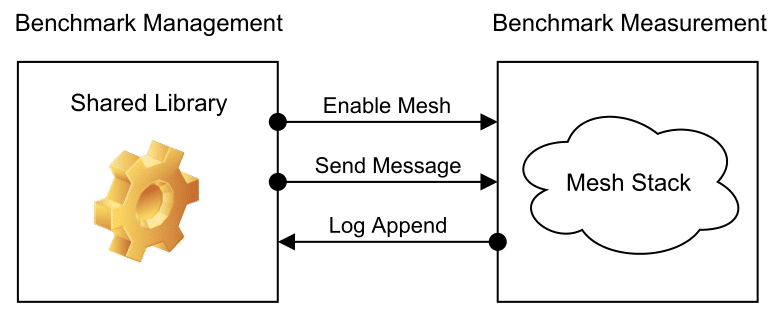
\includegraphics[width=0.6\textwidth]{Shared_Lib_Concept.png}
	\caption{Vereinfachte Anbindung der \textit{Shared Library} an die Mesh-Stacks}\label{fig:ShardeLibConcept}
\end{figure}

\todo[inline]{Schreibfehler in Grafik. measurement statt Meassurment}

Abbildung \ref{fig:ShardeLibConcept} zeigt vereinfacht die Schnittstellen zwischen der Shared-Library und den Mesh-Stacks.
Die Bibliothek ist spezifisch für die nRF52840 SoC's zugeschnitten.
Damit die \textit{Shared-Lib} in die jeweilige SDK integrierbar ist, müssen die enthaltenen Module möglichst ohne weitere Abhängigkeiten auskommen.
Sofern Treiber oder externe Bibliotheken für Module benötigt werden, müssen diese von allen SDKs vergleichbar zur Verfügung gestellt werden.
Im folgenden Abschnitt wird auf die einzelnen Module der \textit{Shared-Lib} eingegangen. 


\subsubsection{Statemachine}\label{subsubsec:StatemachineSoftware}

Die Statemachine dient dazu den Ablauf, welcher in Abschnitt \ref{subsec:AblaufMesh} bereits beschrieben wurde abzuarbeiten. Sowohl der Master als auch die Server und Clients arbeiten den in Abbildung \ref{fig:StatemachineFLowgraph} dargestellten Ablauf ab. 

\begin{figure}[H]
	\centering
	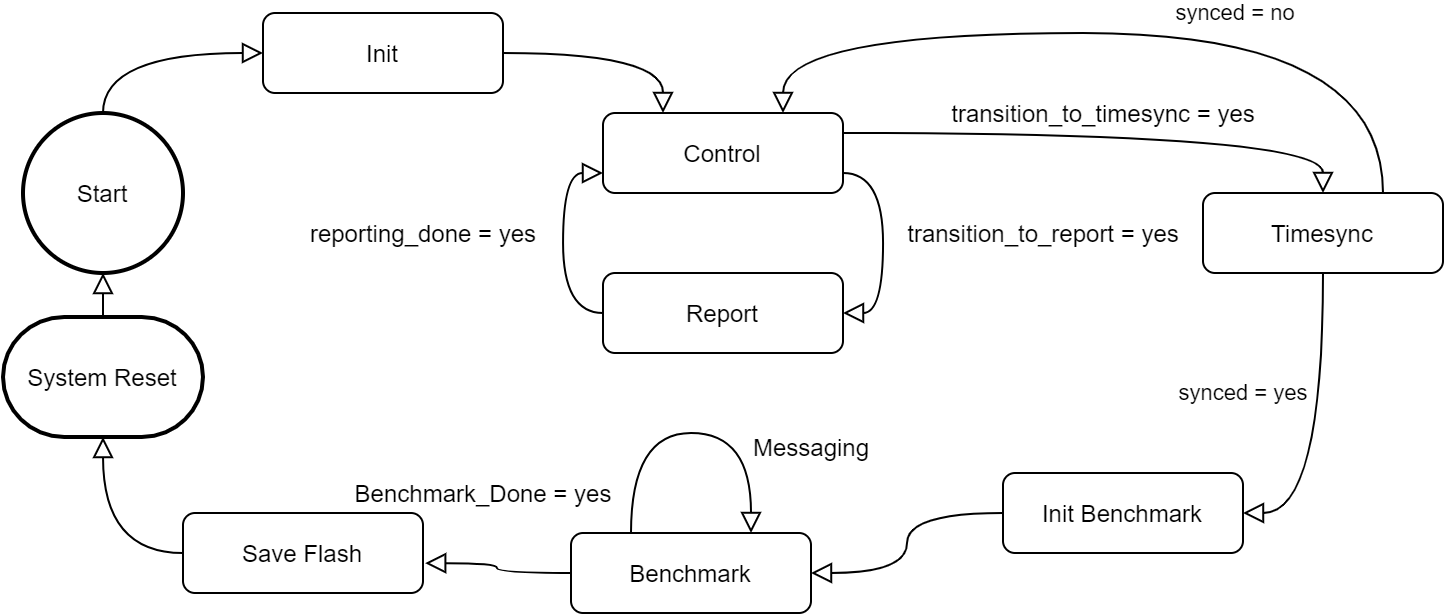
\includegraphics[width=1.0\textwidth]{Statemachine_Flowgraph.png}
	\caption{Flowgraph der Statemachine}\label{fig:StatemachineFLowgraph}
\end{figure}


Die Funktion der Schritte wird nachfolgend grob beschrieben.
\paragraph{Init}
%	\item \textbf{\textit{Init:}}
	Dieser Schritt initialisiert alle notwendige Funktionen (Radio, Timers, usw.). Ebenfalls rekonstruiert er die \textit{Log-Daten} indem er diese aus dem Flash ins RAM lädt. Nach der erfolgreichen Initialisierung wechselt die Statemachine in den Control-State.
	
\paragraph{Control}
%	\item \textbf{\textit{Control:}}
	Im Control-State wartet jeder Teilnehmer auf eingehende Befehle des Benutzers. Der Master erhält über das Command Line Interface (CLI) den auszuführenden Befehl.
	Diesen wandelt der Master in eine Nachricht (Control-Message) um und leitet sie über das Radio-Interface an die Slaves weiter. 
	Alle Slaves (Clients und Servers) erwarten eine Control-Message über das Radio-Interface.
	Damit alle Clients und Servers die Nachricht empfangen können wiederholt jeder Slave jede Control-Message.
	Somit wird die Mesh-Fähigkeit der Verwaltungsschicht (Benchmark Management) sichergestellt.
	Folgende Transitionen sind vom Control-State zugelassen: 
\begin{description}
	\item[\textit{\textbf{Transition to Timesync}}:]
	Wird ein Benchmark gestartet erfolgt dies durch einen Wechsel in den Timesync-State. Jeder Teilnehmer wechselt nach wiederholen der Nachricht in den entsprechenden Schritt. 
	\item[\textit{\textbf{Transition to Report}}:]
	Das Reporting wird über den Report-State abgehandelt. Nur der Teilnehmer von welchem Reports angefordert wurden, wechselt in den Report-State. 
\end{description} 	
	
\paragraph{Timesync}
Der Master verteilt die Zeitsynchronisation an die Slaves. Die Slaves synchronisieren sich auf das Signal des Masters auf, sofern sie in seiner Reichweite liegen. Sobald ein Slave synchronisiert ist, fängt er an die Zeitsynchronisation ebenfalls zu verteilen. Dadurch können Slaves, welche nicht über einen Hop vom Master erreicht werden sich ebenfalls synchronisieren. Konnte ein Slave keine Zeitsynchronisation durchführen, wechselt dieser in den  \textit{Control-State} zurück und bringt einen Fehler mittels der roten-LED zur Anezige. Der Master wird immer zum nächsten Schritt voranschreiten. 	

\paragraph{Init Benchmark}
Im Init Benchmark State werden die Mesh Stacks auf allen Teilnehmern initialisiert und anschliessend gestartet.
Das Netzwerk hat nun Zeit sich aufzubauen, falls dies notwendig ist.
Vor dem Initialisieren des Mesh-Stacks löscht jeder Node die Log-Daten aus dem Flash, sowie dem RAM.
Beim Client wird zusätzlich der Sendezeitpunkt der Benchmark-Nachrichten berechnet und vorbereitet.
Hat sich der Slave erfolgreich initialisiert und mit dem Netzwerk verbunden, leuchtet das grüne Status-LED auf.
Der Wechsel zum Benchmark State wird unabhängig vom Verbindungsstatus nach einer vordefinierten Verzögerungszeit ausgelöst.

\paragraph{Benchmark}
Die Statemachine wartet in diesem Schritt auf die Auslösung von Events.
Beim Server überlässt sie dem Mesh-Stack das Loggen der empfangenen Nachrichten, welcher über einen eigenen Event-Handler verfügt.
Beim Client plant die Statemachine den Versand von Nachrichten mittels Timer-Interrupts.
Löst ein solcher Timer-Interrupt aus, wird der Mesh-Stack unmittelbar benachrichtigt.
Die Erfassung der Logdaten erfolgt ebenfalls im Stack.
Der Status des einzelnen Slaves (Licht EIN / Aus) ist über die grüne RGB-LED (Client) respektive die blaue RGB-LED (Server) erkennbar.
Nach der eingestellten Benchmark-Zeit, löst der Letzte Timer-Interrupt aus und die Abarbeitung des Mesh-Stacks wird unterbrochen.
Es folgt der Wechsel zum letzten Schritt.

\paragraph{Save Flash}
Die erfassten Benchmark Logdaten werden vom RAM ins Flash geschrieben.
Die Speicherung der Log-Daten aus dem im Flash ist notwendig damit diese auch noch einem Neustart persistent bleiben.
Anschliessend wird der Mesh-Stack durch einen Reset des Mikrocontrollers heruntergefahren und neu gestartet.
Dies ist notwendig um sicherzustellen, das der Stack komplett gestoppt ist und das Radio-Interface dem Benchmark Management zur Verfügung steht.
Zudem soll ein neuer Benchmark ohne Vorbelastung gestartet werden können.
Nach dem Reset beginnt die Statemachine automatisch wieder von vorne im Init-State. 

\paragraph{Reports}
Das Einholen von Reports ist nur über eine direkte Verbindung vom Master zum Slave möglich.
Die Übertragung der Log-Einträge erfolgt über ein abgesichertes Handshake-Verfahren.
Der Master sendet eine Anfrage und verlangt beim Slave den n-ten Log-Eintrag.
Der Slave antwortet auf die Anfrage mit dem entsprechenden Log-Eintrag.
Hat der Master diesen erhalten, so verlangt er den nächst höheren Eintrag.
Andernfalls verlangt der Master den selben Eintrage erneut.
Ist die Übetragung zu oft fehlgeschlagen wird das Reporting abgebrochen.
Master wie auch Slave wechseln nach erfolgreichem oder abgebrochenem Reporting in den Control-State.  

\subsubsection{Timesync}\label{subsubsec:Timesync}
Die Zeitsynchronisation wurde identisch wie im Point to Point Teil gemäss Abschnitt \ref{sec:ZeitsynchronisationP2P} umgesetzt.
Durch die Wiederholung der Master-Timestamps bei jedem Hop, nimmt der Synchronisationsfehler stetig zu.
Angenommen pro Hop entsteht ein maximaler Fehler von 1.2$\mu$s, so wäre der maximale Fehler nach sieben Hops bereits 8.4$\mu$s gross.
Dieser Fehler ist noch immer vernachlässigbar klein verglichen mit dem Clock-Drift der zusätzlich vorhanden ist.
Die Genauigkeit des Quarz-Oszilators auf dem nRF52840 liegt bei $\pm$ 10ppm \cite{nordic_semiconductor_asa_nrf52840_ps_v11pdf_nodate}.
Das ergibt pro Sekunde ein maximalen Clock-Drift von 20$\mu$s. 

Um die Funktionen von Master und Slave zu unterscheiden, wurde eine Subscribe- sowie eine Publish-Funktion definiert.
Der Master verteilt den Timestamp über die Publish-Funktion.
Der Slave reagiert auf Timesync-Pakete mittels Subscribe Funktion.
Erhält der Slave ein Timesync-Paket, wiederholt dieser das Frame mittels Publish-Funktion.
Vor dem weiterleiten mittels Pusblish muss ein zufälliger Timeslot abgewartet werden, damit es nicht zu Kollisionen zwischen den Timesync-Paketen kommt.
Die maximale Backoff-Zeit wird gemäss Abschnitt \ref{sec:BroadcastingCollissionsProbability} berechnet.
Dementsprechend muss das Zeitfenster zur Synchronisation genügend lang sein, damit sich alle Teilnehmer synchronisieren können.

Ein Timesync-Paket setzt sich aus folgenden Feldern zusammen: 

\begin{itemize}
\item \textit{uint64\_t} \textbf{LastTxTimestamp:}
	Gibt den Zeitstempel (Master-Zeit) an welcher zum Versandzeitpunkt des Probepakets erfasst wurde.
\item \textit{uint64\_t} \textbf{NextState\_TS\_us:}
	Definiert den Zeitpunkt um in den nächsten Schritt zu wechseln.
\item \textit{uint32\_t} \textbf{MAC\_Address\_LSB:}
	Die Identifizierung des Time-Masters. Muss mit jener Addresse des zuvor empfangenen Pakets übereinstimmen.
\item \textit{uint8\_t} \textbf{seq:}
	Aufsteigende Nummer um jedes Times-Sync Paket zu identifizieren. Der Slave prüft ob das eingehende Paket das direkt Folgende des zuvor erhaltenen Pakets ist.
\end{itemize}


\footnotetext{\url{https://github.com/Rouben94/P6_Software/blob/master/SharedLib/bm_timesync.c} \cite{rouben94_sharedlib_timesync_software_git_2020}}

\subsubsection{Control}\label{subsubsec:Control}
Im Control State befinden sich alle Teilnehmer in Bereitschaft wie bereits in Abschnitt \ref{subsubsec:StatemachineSoftware} beschrieben.
Analog zu den im Abschnitt \ref{subsubsec:Timesync} definierten Publish- und Subscribe-Funktionen wurden solche auch für die Verteilung der Control-Messages definiert.
Eine Control-Message beinhaltet die folgenden Felder:

\begin{itemize}
	\item \textit{uint32\_t} \textbf{MACAddressDst:} Control-Messages erfüllen den Zweck den Zustand eines Teilnehmers oder den aller Teilnehmer zu ändern.
Dazu wurde dieses Feld als Ziel MAC-Adresse festgelegt. Die MAC-Adresse 0xFFFFFFFF ist als Broadcast definiert.
	
	\item \textit{uint8\_t} \textbf{depth:} Depth steht für die Anzahl Relays die die Nachricht bereits passiert hat.
	Der Master sendet immer mit der Depth 0.
	Wird ein Paket relayed (wiederholt) wird das Depth-Feld inkrementiert.
	Empfängt der Node ein Paket mit einer Depth die höher ist als jene des zuletzt empfangenen Pakets, so wird das Paket nicht erneut gesendet.
	Die zuletzt empfangene Depth ist nur eine gewisse Zeit gültig um auf Veränderungen im Netzaufbau reagieren zu können.
	Abbildung \ref{fig:ControlMessagesHops} zeigt die Verbreitung einer Control Message mithilfe des Depth-Feldes.
	
	
\begin{figure}[H]
\centering
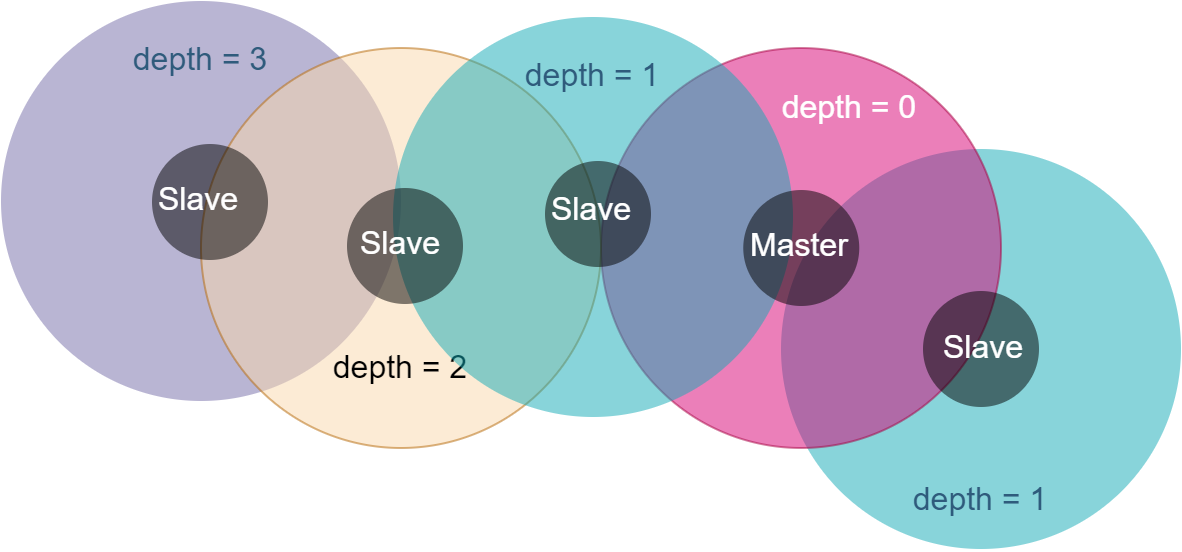
\includegraphics[width=0.8\textwidth]{Control_Hops.png}
\caption{Konzept des Depth-Feld beim Versand einer Control Message}\label{fig:ControlMessagesHops}
\end{figure}

	
	\item \textit{div.} \textbf{Control-Paramter} Die restlichen Felder sind Parameter welche den Zustand des Nodes verändern oder Parameter übergeben. 
\end{itemize}


Ein Teilnehmer signalisiert über aufblinken der grünen-LED seine Bereitschaft um weitere Control Messages verarbeiten zu können. Blinkt die blaue-LED auf zeigt dies an das der Teilnehmer eine Zustands- oder Parameteränderung erhalten hat. 

Das Abfragen von Control-Messages erfolgt durch Pollen.
Dies hat den Ursprung, das nicht bei allen SDK's der Interrupt des Radio-Interfaces frei ist.


\subsubsection{Report}\label{subsubsec:Report}

Wie bereits in Abschnitt \ref{subsubsec:StatemachineSoftware} beschrieben, versendet der Master Anfragen an einen Slave um dessen Reports einzuholen.
Dazu wird eine Control-Message vom Master initiiert um den Slave in den Reporting Zustand zu versetzen.
Diese Nachricht wird zwar relayed jedoch funktioniert das anschliessende Reporting nur über eine direkte Verbindung.

Das Reporting teilt sich in eine Subscribe und Publish-Funktion auf.
Der Master subcribed auf Reports und sendet Report Requests an den Slave.
Der Slave erwartet in der Publish-Funktion Report-Requests des Masters.
Erhält ein Slave einen Request, so antwortet er dem Master mit dem verlangten Eintrag.

\begin{figure}[H]
	\centering
	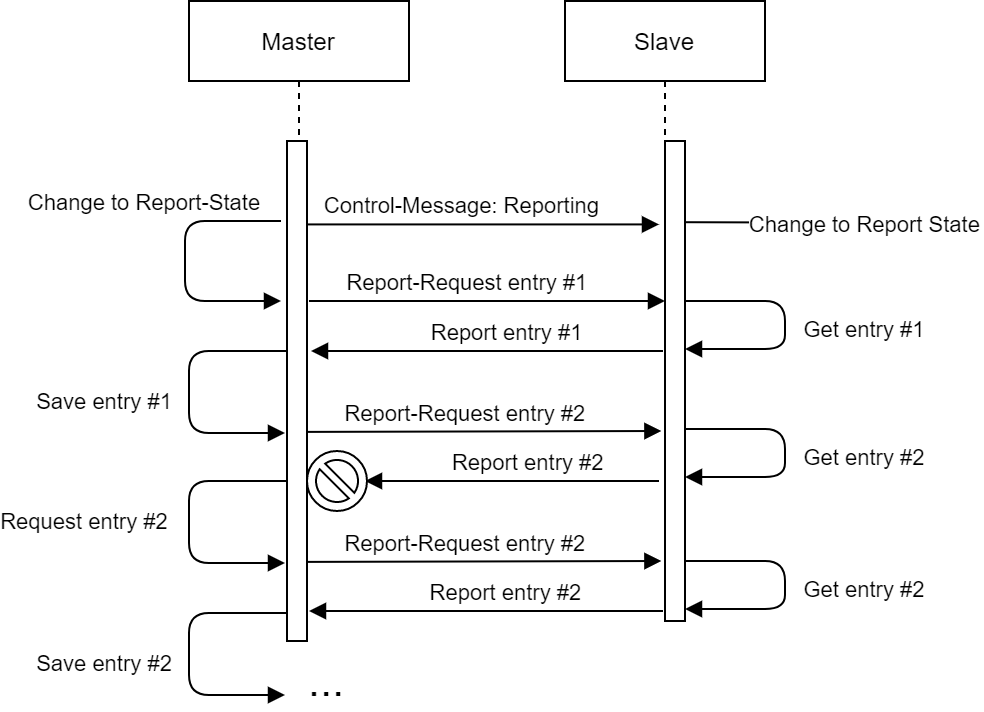
\includegraphics[width=0.9\textwidth]{Reporting_Flowchart.png}
	\caption{Ablauf des Reportings mit Handshake zwischen Master und Slave}\label{fig:ReportingAblauf}
\end{figure}

Die Abbildung \ref{fig:ReportingAblauf} zeigt den Ablauf des Reportings beispielhaft.
Mithilfe des Handshake Verfahren (siehe Abschnitt \ref{subsubsec:StatemachineSoftware}) wird der Report-Entry 2 nochmals angefordert, da dieser nicht erfolgreich beim Master angekommen ist.

Sobald der Report als ungültig erkannt wird, wird das Reporting beidseitig beendet.
Dies geschieht durch die Prüfung des Zeitstempel-Feldes des jeweiligen Report Eintrages auf den Wert Null.
Falls keine Verbindung zustande kommt, brechen Master sowie Slave nach einer bestimmten Anzahl von Versuchen das Reporting ab.


\subsubsection{Logging}\label{subsubsec:Logging}
Das Logging-Modul ist für die Verwaltung der Log-Daten im RAM sowie im FLASH zuständig.
Es definiert das Format eines Log-Eintrages welcher bereits in Abschnitt \ref{subsubsec:Messgrössen} vorgestellt wurde.
Die Länge eines Eintrages erreicht eine Grösse von 28 Byte.
Sämtliche Einträge werden durch das Modul als Array mit 3000 Log-Einträgen gespeichert.
Diese Konstante Array Grösse kommt folgendermassen zustande.
Pro Client können maximal 1000 Nachrichten verschickt werden.
Ein Server soll mit maximal drei Clients in der selben Gruppe sein.
Damit er alle Einträge aufnehmen kann, wurde die Länge des Arrays auf 3000 festgelegt.
Somit müssen 84kByte RAM und Flash für das Log zur Verfügung stehen. Die im Ablauf benötigten Funktionen des Moduls lassen sich folgendermassen beschreiben. 

\begin{itemize}
	\item \textit{\textbf{bm\_log\_clear\_ram():}} Wird genutzt um alle Log-Einträge aus dem RAM zu entfernen.
	\item \textit{\textbf{bm\_log\_append\_ram():}} Fügt einen Log-Eintrag dem RAM hinzu. Das Modul verwaltet selbst den nächsten freien Index. 
	\item \textit{\textbf{bm\_log\_clear\_flash():}} Bewirkt ein Löschen des gesamten Logs im FLASH. 
	\item \textit{\textbf{bm\_log\_save\_to\_flash():}} Schreibt den gesamten Log vom RAM in das FLASH. 
	\item \textit{\textbf{bm\_log\_load\_from\_flash():}} Lädt den gesamten Log vom FLASH in das RAM. 
	\item \textit{\textbf{bm\_log\_init():}} Initialisiert das Logging-Modul.
\end{itemize} 

Die Abarbeitung des Flash Moduls wurde bei Zephyr direkt in diesem Log-Modul integriert.
Handelt es sich um eine nRF-SDK findet das Handling des Flashs in einem separaten Modul statt (siehe Abschnitt \ref{subsubsec:FlashSave}).

Zephyr organisiert die Flash-Bereiche mithilfe eines Device-Tree-Source-Files (DTS).
Darin werden verschiedene Partitionen definiert.
Die Partition in welchen die Daten gespeichert werden, ist vom Bootloader für ein DFU-Upgrade reserviert.
Sofern kein DFU-Upgrade im Gange ist kann der Bereich beliebig genutzt werden. Die Partition muss mindestens 84kByte zur Verfügung stellen.
Der Zugriff auf das Flash ist über das Zephyr OS geregelt welches einen Flash-Treiber zur Verfügung stellt.
Dieser kann eine Pages-Grösse von 4kByte löschen. 


\subsubsection{Flash Save}\label{subsubsec:FlashSave}
Das Modul Flash Save wird zur Speicherung von Daten im FLASH benutzt.
Dies geschieht mit Hilfe der Flash-Device-Storage (FDS) API, welche in der \textit{nRF SDK for Mesh}, sowie in der \textit{nRF SDK for Thread and Zigbee} angeboten wird.
Sie erlaubt die Speicherung von Daten im Flash und implementiert ein \textit{Basic-Wearleveling}.

Das FDS-Modul beginnt, falls nicht anders vorgesehen, direkt unterhalb der Bootloader-Adresse mit der Speicherung der Daten im Flash.
Mittels der \textit{sdk-config.h} Konfiguration werden die Länge des Flash-Bereichs und weitere Einstellungen für das FDS-Modul festgelegt.
Die abzuspeichernden Daten werden in Records unterteilt.
Zur Abspeicherung der Log-Daten wurde nur ein Record verwendet \cite{nordic_semi_nrf5_sdk_flash_data_storage_2020}.



\subsubsection{CLI}\label{subsubsec:CLI}
Mit diesem Modul werden Ein- / Ausgaben über das Command-Line-Interface (CLI) ermöglicht.
Die einfachste Funktionalität ist die Ausgabe über einen Log-Befehl.
Dieser ist mittels \textit{bm\_cli\_log("Hello")} aufrufbar.
Das Kommando wird auf die jeweilige Umgebung (SDK) angepasst.
Bei den \textit{nRF SDK's} werden Logs mittels dem \textit{NRF\_LOG()} Befehl, bei \textit{Zephyr} mittels \textit{printk()} ausgegeben.

Die zentrale Funktionalität des Moduls bezieht sich auf die Verarbeitung von CLI-Befehlen.
Dafür werden verschiedene CLI-Befehlssätze angeboten, welche im Sub-Modul \textit{bm\_cli\_cmds.c} definiert sind.

\begin{itemize}
	\item \textit{\textbf{setNodeSettings:}} Mithilfe dieses Befehlssatzes können die Einstellungen eines Slaves (Server/Clients) geändert werden. Eine Eingabe muss folgendes Format haben:
	\textit{setNodeSettings <MAC in Integer format> <GroupNumber> <Node Id> <Ack> <AdditionalPayloadSize> <BenchmarkTrafficGenMode> <DST\_MAC\_1> \linebreak <DST\_MAC\_2> <DST\_MAC\_3>}.
	Die Bedeutung der einzelnen Felder sind in Abschnitt \ref{MeshBenchmarkKonzeptundTestumgebung} angedeutet.
	\item \textit{\textbf{getNodeReport:}} Mithilfe dieses Befehlssatzes können die Reports eines Slaves (Server/Clients) abgefragt werden. Eine Eingabe muss folgendes Format haben: 
	\textit{getNodeReport <MAC in Integer format>}. Die Bedeutung der einzelnen Felder sind in Abschnitt \ref{subsubsec:NodeIdentification} angedeutet. 
	\item \textit{\textbf{startBM:}} Mithilfe dieses Befehlssatzes wird ein Benchmark gestartet. Eine Eingabe muss folgendes Format haben:
	\textit{startBM <BenchmarkTime (seconds)> <BenchmarkPacketsCount>}. Das erste Feld gibt die Benchmark Zeit in Sekunden an. Beim zweiten Feld handelt es sich um die Anzahl Nachrichten welche versendet werden sollen. 
\end{itemize}

Erhält der Master eine der oben erwähnten Befehlssätze löst dieser eine entsprechende Control-Message aus.
Die zugewiesenen Parameter werden ebenfalls mithilfe des Moduls abgespeichert und initialisiert. 


\subsubsection{Traffic Generator}\label{subsubsec:TrafficGenerator}
Im folgenden Modul werden die Sende-Zeitwerte von Nachrichten generiert.
Das Konzept dazu wurde bereits in Abschnitt \ref{subsec:TrafficGeneration} erläutert.
Dabei wird zwischen zufälligen und sequentiellen Werten unterschieden.  

Wird eine Messung mit sequentiellen Werten gestartet erstellt dieses Modul, abhängig von den Benchmark-Parametern, eine Abfolge gemäss der bereits erwähnten Formel \ref{eq:TrafficGenerationSeq}.

Wird eine Messung mit zufälligen Werten gestartet erstellt dieses Modul, abhängig von den Benchmark-Parametern, ein neu generiertes Set oder verwendet ein bereits vorhandenes Set an zufälligen Werten.
Es existieren 25 verschiedene vordefinierte Sets welche vorgängig über die Webseite \textit{random.org\footnote{\url{https://www.random.org/}}} erzeugt wurden.
Die Einstellungen, welche zur Erzeugung der Werte verwendet wurden, sind im Anhang \ref{app:RandomTrafficGeneration} zu finden.

Wurde ein Set festgelegt werden diese Werte mittels eines \textit{Bubble-Sort} Algorithmus in aufsteigender Reihenfolge sortiert.
Anschliessend müssen die Werte auf den Zeitbereich des Benchmarks skaliert werden.
Da es isch bei den zufällig generierten Werten um \textit{uInt16} Datentypen handelt liegt der Wertebereich zwischen 0-65535.
Die Werte werden gemäss Formel \ref{eq:TrafficGenerationRand} berechnet. 

\begin{equation}\label{eq:TrafficGenerationRand}
T_{Msg\_send} =  \frac{V_{Rand}}{UINT16MAX} \cdot T_{Benchmark}
\end{equation}

\begin{small}
	\begin{center}
		\begin{tabular}{ll}
			$T_{Msg\_send}$ & Zeitpunkt zu welchem die Nachricht gesendet wird.\\
			$T_{Benchmark}$ & Benchmark Dauer (siehe \ref{tab:ParameterBenchmarkMessreihe})\\
			$V_{Rand}$ & Random Value aus dem Set \\
			$UINT16MAX$ & Maximaler Wert des UInt16 (65535) \\
		\end{tabular}
	\end{center}
\end{small}

\subsubsection{Low Level Radio}\label{subsubsec:LowLevelRadio}
Der Low-Level-Radio Treiber soll möglichst unabhängig direkt mit dem Radio-Interface operieren.
Er stellt die für die Verwaltung der Messung notwendigen Funktionen zur Verfügung.
Senden oder Empfangen von Daten sollen mittels einfachen Aufrufen möglich sein.

Das Radio-Interface wird beinahe identisch zur P2P-Testinfrastruktur bedient (siehe Abschnitt \ref{sec:LowLevelRadioDriver}).
Lediglich auf die Verwendung von Interrupts musste verzichtet werden, da die meisten Radio-Driver der Mesh-Stacks diese bereits belegt haben.
Insbesondere beim Zephyr findet die Initialisierung des Radio-Drivers vor dem Aufrufen der Statemachine statt.
Somit wurden die Events durch Pollen abgefragt.


\subsection{Benchmark Management}\label{subsec:Benchmark Management}

Um die Verwaltung einer Messung zu automatisieren stehen folgende Python-Scripts zur Verfügung.
Die Scripts werden auf der BMS (Benchmark Management Station) ausgeführt.
Die Konfiguration der Teilnehmer wird mittels einem Excel-File durchgeführt (siehe Abschnitt \ref{subsubsec:NodeConfiguration}). 


\subsubsection{Flasher}\label{subsubsec:Flash}
Dieses Script dient dazu alle nRF52-Dongles mit der entsprechenden Firmware zu flashen.
Dazu liest das Script die Konfigurationsdatei aus.
Mithilfe der dort vorhanden Informationen fordert das Script den Benutzer dazu auf den Dongle mit der entsprechenden Nummer via USB Buchse mit dem PC zu verbinden.
Sobald der Dongle eingesteckt wurde beginnt das Script mit dem Flashen.
Dies geschieht mit Hilfe des nrfutil-Tools. 

\subsubsection{Configurator}\label{subsubsec:Configurator}
Mithilfe des Configurator-Scripts kann eine voreingestellte Konfiguration auf die einzelnen Teilnehmer verteilt werden.
Das Script arbeitet die Konfigurations-Einträge der Reihe nach ab.
Mittels dem an der BMS angeschlossenen Masters versendet das Script den entsprechenden Konfigurationsbefehl. 

\subsubsection{Benchmark and Reporter}\label{subsubsec:BenchmarkandReporter}
Über dieses Script wird entweder eine Messung gestartet oder die Resultate einer vorhergehenden Messung eingeholt.
Wird ein neuer Benchmark initiiert muss der Benutzer die Benchmark-Parameter angeben.
Anschliessend startet das Script über den angeschlossenen Master den Vorgang.
Während der Messung zeigt das Script die Meldungen des Masters an.

Nach Abschluss der Messung können die Reports mithilfe des Scripts eingeholt werden.
Dazu fordert das Script den Benutzer auf sich in die Nähe des ersten Slaves zu begeben.
Nach der Bestätigung beginnt das Script damit die Daten des Slaves einzusammeln.
Nach dem Einsammeln aller Daten der Slaves schreibt das Script die Werte in ein CSV-File. 

%\subsubsection{Analysis}\label{subsubsec:Analysis}
%Sind alle Report-Daten in einem Excel-File abgespeichert, können die Messgrössen mithilfe des Analysis-Scripts berechnet werden.
%Dieses wertet die einzelnen Daten aus und stellt die Messdaten in einem ergänzenden CSV-File zur Verfügung.
%Dieses Script wird nicht länger benötigt da die Auswertung neu komplet in Excel erfolgt. 

